\setcounter{page}{1} \pagenumbering{Alph}

% Add PDF bookmark 
\pdfbookmark[0]{Title}{Title}

%%% LOGO
\thispagestyle{empty}
\begin{flushleft} ~\\ \vspace{-12mm} \hspace{-12mm}  
\includegraphics[width=50mm]{Cover/istnewlogo}

    %%% Instituição
    \centering
    \LARGE \textbf{UNIVERSIDADE DE LISBOA \\ INSTITUTO SUPERIOR TÉCNICO}
    %%% espaço sem gráficos
    \vspace{30mm}

    %%% Optional Image
    %\vspace{10mm}
    %~\\ \vspace{50mm} % gráficos
    %\\ \begin{center} 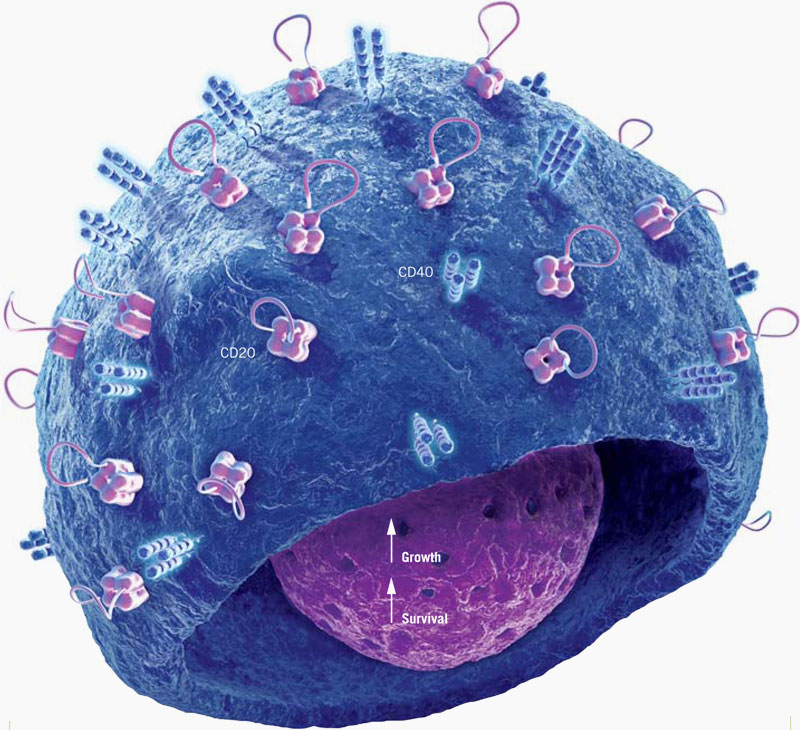
\includegraphics[height=50mm]{Cover/coverimage}  \end{center} % gráficos
    % \vspace{5mm}

    %%% Titulo
    \centering
    \LARGE \textbf{Learnable Sparsity and Weak Supervision\\for Data-Efficient, Transparent, and Compact\\Neural Models}
    %\\ \vspace{10mm}
    %\Large Optional Subtitle
    %\\ \vspace{15mm}
    \\ \vspace{25mm}  % NO SUBTITLE
    \LARGE \textbf{Gonçalo Migueis de Matos Afonso Correia} \\
    \vspace{25mm}

    %Advisors
    \Large %letter size for advisers
    \begin{minipage}{\textwidth}
        \hspace{10mm}
        \begin{tabularx}{\textwidth}{ l @{ } l }
            \centering
            \textbf{Supervisor} :    & Doctor André Filipe Torres Martins \\
            \textbf{Co-Supervisor} : & Doctor Vlad Niculae                \\
        \end{tabularx}
    \end{minipage}
    %
    \\ \vspace{20mm}
    \centering
    \Large \textbf{Thesis approved in public session to obtain the PhD Degree in}\\
    \Large \textbf{Electrical and Computer Engineering}\\
    \vspace{10mm}
    \Large \textbf{Jury final classification:  Pass with Distinction and Honour}\\
    \vspace{20mm}

    \Large \textbf{2022} \\
    \let\thepage\relax
\end{flushleft}
\pagebreak
